\documentclass{apuntes}

\title{Automatas y lenguajes}
\author{Pedro Valero}
\date{14/15 C1}

% Paquetes adicionales

% --------------------

\begin{document}
\pagestyle{plain}
\maketitle

\tableofcontents
\newpage

\printindex

\chapter{Introducción}
Vamos a trabajar con tres elementos fundamentales:
\begin{itemize}
\item \textbf{Máquinas/Autómata}
\begin{itemize}
\item Autómatas finitos $\Rightarrow$ Expresiones regulares
\item Autómatas de pila $\Rightarrow$ Lenguajes libres de contexto
\end{itemize}
\item \textbf{Problemas} ¿Qué se puede computar?. Conjeturas que se creen ciertas pero cuya veracidad, por ahora, no se ha demostrado.

\item \textbf{Lenguajes/Gramática}
\end{itemize}

Nuestro objetivo es ver que relacion existe entre estos tres elementos. Para ello, primero debemos establecer algunas definiciones.

\section{Lenguaje}
\begin{defn}[Símbolo]
``Letra", elemento de un conjunto
\end{defn}

\begin{defn}[Alfabeto]
Conjunto finito de símbolos no vacío.
\end{defn}

\begin{defn}[Palabra (Cadena)]
Secuencia finita de símbolos tomados de un alfabeto.
La palabra vacía se representa por $\lambda$
\end{defn}
Será conveniente acostumbrarnos a usar el término ``cadena" en lugar del término ``palabra" ya que representa mejor el concepto que queremos representar.


\begin{defn}[Longitud de cadena]
Número de símbolos que contiene
\end{defn}

\begin{defn}[Lenguaje]
Conjunto de palabras
\end{defn}

Hay algunos casos particulares de lenguajes:
\subsection{Lenguajes particulares}
\begin{defn}[Lenguaje universal (sobre $\sum$)]
Denotado por $\sum^*$ representa el conjunto de todas las palabras que se pueden formar
\end{defn}

\begin{defn}[Lenguaje de un autómata]
Conjunto de palabras que acaban en un estado final del autómata son aceptadas por el mismo)
\end{defn}

\begin{defn}[Lenguaje vacío]
Lenguaje que no contiene ningún elemento
\end{defn}

\begin{defn}[Lenguaje $\lbrace \lambda \rbrace$]
Lenguaje que sólo contiene $\lambda$.
\end{defn}
El lenguaje $\lbrace \lambda \rbrace$ es distinto del lenguaje vacío aunque $\lambda$ sea la palabra vacía.

\subsection{Operadores de utilidad}
Añado esta sección ya que el profesor lo ha aclarado en ningún momento ni parece tener intención de hacerlo.

Tenemos dos operadores importantes:
\begin{enumerate}
\item \begin{defn}[Estrella]
El operador estrella se corresponde con la suma infinita:
\[a^* = 0 + a + a^2 + a^3 + ...\]
Donde el 0 implica que esa ``a" no aparece ninguna vez. Según en que cuerpo nos moviésemos podrá tener distinto significado. Técnicamente sería el elemento nulo de la suma.
\end{defn}
\item \begin{defn}[Suma]
Este operador se corresponde con la suma infinita:
\[a^* = a + a^2 + a^3 + ...\]
(El nombre de este operador no lo tengo claro en castellano)
\end{defn}
\end{enumerate}
Estos conceptos nos sirven para entender por qué $\Sigma ^*$  representa todas las palabras posibles. Para poder entender esto debemos entender la multiplicación como una concatenación y la suma como un \textit{OR}. Así el ```elemento neutro de la suma" sería la cadena vacía.

Tomemos ahora el alfabeto binario $\Sigma = \lbrace 0, 1 \rbrace$
Entonces:
\[\Sigma ^* = (0+1)^* = \emptyset + (0+1)+(0+1)^2+(0+1)^3+... = \]
\[= \emptyset + 0 + 1 + 00 + 01 +10 +11 +000+001+010+011+100+101+110+111+...\]
Y con esto vemos como se forman todas las posibles combinaciones de bits de diferente longitud. Si en lugar de este alfabeto hubiésemos tomado nuestro alfabeto castellano habríamos obtenido todas las posibles combinaciones de letras.

\section{Gramática}
\begin{defn}[Gramática]
Hay varias definiciones para este término. No son muy precisas pero nos dan una idea de su significado:
\begin{enumerate}
\item Mecanmismo para formalizar matemáticamente un lenguaje
\item Conjunto de reglas que determinan cómo formar las cadenas de un lenguaje
\end{enumerate}
\end{defn}

\begin{example}
Tomemos las reglas:
\begin{enumerate}
\item ORACIÓN $\Rightarrow$ SUJETO + PREDICADO
\item SUJETO $\Rightarrow$ ARTÍCULO + NOMBRE
\item PREDICADO $\Rightarrow$ VERBO
\item ARTÍCULO $\Rightarrow$ el ó un
\item NOMBRE $\Rightarrow$ coche ó perro
\item VERBO $\Rightarrow$ come ó corre
\end{enumerate}
Estas reglas constituyen una gramática que nos permite generar un lenguaje. En este caso el lenguaje estaría formado todas las cadenas que se pueden construir a partir de estas reglas
%TODO Ejemplo de árbol de derivación con estas reglas
\end{example}

\begin{defn}[Símbolos terminales]
Símbolos que pueden aparecer en la cadena final. En el ejemplo anterior serían elementos terminales aquellos escritos en minúscula. Para ellos no existe ninguna regla que indique cómo se derivan.
\end{defn}

\begin{defn}[Símbolos no terminales]
Símbolos que no pueden aparecer en la cadena final. Simplemente son usados para definir las reglas de derivación
\end{defn}

\begin{defn}[Reglas de producción]
Explican cómo se transforma un símbolo no terminal en un conjunto de símbolos terminales o no terminales
\end{defn}

\begin{defn}[Símbolo inicial / Axioma]
Indica dónde empieza a construirse la cadena. En el ejemplo anterior, el axioma sería el símbolo ORACIÓN. Una gramática sólo puede tener un úncio axioma.
\end{defn}

Vamos a ver algunos ejemplos de gramáticas y los lenguajes que generan:
\begin{example}
Tomemos la gramática:
\begin{enumerate}
\item S $\Rightarrow$ aSb
\item S $\Rightarrow$ $\lambda$
\end{enumerate}

El lenguaje generado por esta gramática serían todas las palabras de la forma: $a^i\lambda b^i$ con $ i=0,1,... \infty$
\end{example}

\begin{example}
Ahora vamos a tratar de construir la gramática que define un lenguaje dado:
L(G)=$\lbrace a^nb^{n+1}, n \geq 0 \rbrace$

La gramática que define este lenguaje es:
Tomemos la gramática:
\begin{enumerate}
\item S $\Rightarrow$ aSb
\item S $\Rightarrow$ b
\end{enumerate}

El automata asociado a este lenguaje sería:
\begin{center}
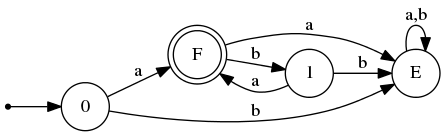
\includegraphics[scale=0.75]{automata1.png}
\end{center}
\end{example}

\begin{defn}[Lenguajes Regulares]
Son lenguajes que pueden ser admitidos por autómatas finitos
\end{defn}

\begin{defn}[Gramáticas libres de contexto]
Son aquellas donde a la izquierda sólo aparece un único símbolo no terminal
\end{defn}


\begin{example}[Gramática dependiente de contexto]
\begin{itemize}
\item aSb $\Rightarrow$ abb
\item cSd $\Rightarrow$ cdd
\end{itemize}
S puede derivarse dependientemente de lo que la rodee, es decir, de su contexto
\end{example}

\begin{example}[Gramática independiente de contexto (regular)]
\begin{itemize}
\item A $\Rightarrow$ aA
\item A $\Rightarrow$ a
\end{itemize}
A la derecha tenemos únicamente símbolos terminales o bien símbolos terminales acompañados de un único símbolo no terminal.
Si el elemento no terminal está a la izquierda se denomina gramática lineal por la derecha. En caso contrario, gramática lineal por la izquierda
\end{example}

\begin{defn}[Equivalencia de gramáticas]
Dos gramáticas son equivalentes si generan el mismo lenguaje
\end{defn}

\chapter{Autómatas}
\begin{defn}[Automata]
Se representa como:
\[ A=(Q, \Sigma, \delta, q_0, F)\]
 donde:
\begin{itemize}
\item Q = conjunto de estados
\item $\Sigma$ =  alfabeto de entrada
\item $\delta$ = función de transición: $\delta : Q\times \Sigma \rightarrow Q$
\item $q_0$ = estado inicial
\item F = conjunto de estados finales
\end{itemize}
\end{defn}

\begin{defn}[Automata Determinista. AFD\IS]
Implica que la función de transición es inyectiva. Dado un estado y una entrada sólo hay un estado al que podamos pasar.
\[\delta: Q \times \Sigma \rightarrow Q\]
\end{defn}

\begin{defn}[Función de transición extendida\IS]
Consiste en una extensión de la función de transición a cadenas. Se representa como $\delta ^*$:
\[\delta^*(q, w)=q_1\]
Siendo $w\in \Sigma ^*$, $q$ el estado en el que comenzamos y $q_1$ el estado al que llegamos tras parsear toda la palabra.
\end{defn}

\newpage

\begin{defn}[Lenguage aceptado\IS por un AFD]
El lenguage aceptado por un automata finito determinista, A, es el conjunto de palabras que llevan al autómata al estado final.
\[L(A) = \lbrace w \in \Sigma^* \ : \ \delta^*(q_0, w) = F \rbrace\]
\end{defn}

Veamos algún ejemplo:
\begin{example} 
Queremos un autómata que reconozca el lenguaje: L=$\lbrace$101,110$\rbrace$

El automata resultado es:
\begin{center}
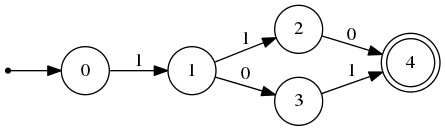
\includegraphics[scale=0.75]{automata2.png}
\end{center}

Este autómata es determinista, pero podríamos representar el mismo lenguaje con un autómata no determinista:

\begin{center}
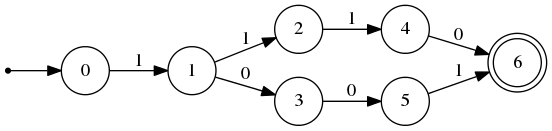
\includegraphics[scale=0.75]{automata3.png}
\end{center}

La ventaja de un autómata no determinista es que podemos explorar varias ramas en paralelo.
\end{example}

\begin{defn}[Transición $\lambda$]
Transición que puede ocurrir sin recibir ningún valor de entrada. Un autómata que desde un estado pueda moverse leyendo algún valor o con una transición de este tipo se considera no determinista
%TODO Comprobar si basta con transición landa para no deterministmo.
\end{defn}

\begin{defn}[Automata finito no determinista. AFN\IS]
Automata con función de transición de la forma:
\[\delta: Q\times (\Sigma \cup \lbrace \lambda \rbrace) \rightarrow 2^Q\]
Es decir, dado un estado y una entrada posiblemente vacía salto a un conjunto de estados.
\end{defn}

\begin{defn}[Función de transición extendida\IS]
Consiste en una extensión de la función de transición a cadenas. Se representa como $\delta ^*$:
\[\delta^*(q, w) = E\]
Siendo $w\in \Sigma ^*$, $q$ el estado en el que empezamos y $E$ el conjunto de estados a los que llegamos tras parsear toda la palabra.
\end{defn}

\begin{defn}[Lenguage aceptado\IS por un AFN]
El lenguage aceptado por un automata finito no determinista, A, es el conjunto de palabras que llevan al autómata a un estado final.
\[L(A) = \lbrace w \in \Sigma^* \ : \ \delta^*(q_0, w)\cap F \neq \emptyset \rbrace\]
\end{defn}

\begin{example}
Diseñar un autómata para el siguiente lenguage

Tenemos el alfabeto: $\Sigma = \lbrace 0,1,2,3,4,5,6,7,8,9,+,-,\cdot \rbrace$ con las siguientes restricciones:
\begin{enumerate}
\item Signo puede o no aparecer
\item Parte decimal puede aparecer o no
\item Parte entera puede o no aparecer
\item Debe haber al menos parte entera o decimal.
\end{enumerate}

El autómata queda:
\begin{center}
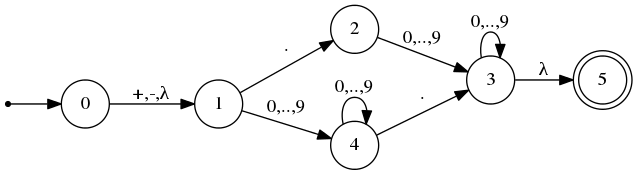
\includegraphics[scale=0.75]{automata4.png}
\end{center}
Siendo L la transición $\lambda$
\end{example}

\chapter{Expresiones regulares}
\begin{defn}[Expresión regular]
Forma alternativa de representar un lenguage regular
\end{defn}

Dado un alfabeto $\Sigma$ existen tres tipos de expresiones regulares primitivas:
\begin{enumerate}
\item $\emptyset$ 

L($\emptyset$) = $\emptyset$
\item $\lambda$

 L($\lambda$)=$\lbrace \lambda \rbrace$
\item $a\in \Sigma$ 

L($a$) = $\lbrace a \rbrace$
\end{enumerate}

A partir de estas expresiones regulares primitivas podemos construir expresiones regulares complejas aplicando la siguiente regla

Siendo $\alpha, \beta$ dos expresiones regulares primitivas o compuestas sobre $\Sigma$ también lo son:
\begin{enumerate}
\item $\alpha + \beta$ (Unión de lenguages)

L($\alpha + \beta$) = L($\alpha $) $\cup$ L($\beta$)
\item $\alpha . \beta$ (Concatenación de lenguages)

L($\alpha . \beta$) = L($\alpha $). L($\beta$)
\item $\alpha^*$ (Cierre)

L($\alpha^*$) = L($\alpha$)$^*$
\item $\beta^*$ (Cierre)

L($\beta^*$) = L($\beta$)$^*$
\end{enumerate}

\section{Equivalencia entre AF y ER}
Vamos a ver cual es la relación existente entre los autómatas finitos y las expresiones regulares.

Como ya vimos una gramática regular puede expresarse como una cuádrupla G=(N,T,S,R), es decir, consta de símbolos no terminales, símbolos terminales, un símbolo inicial o axioma y unas reglas de producción.

Recordamos también que una gramática regular es aquella que es lineal por la derecha o lineal por la izquierda
 
Hay 4 formas de representar un lenguage regular, y en ellas reside la equivalencia entre Autómatas finitos y expresiones regulares. Las 4 formas de representar un lenguage regular son:
\begin{enumerate}
\item Describiendo todos sus componentes
\item Con una gramática regular
\item Con una expresión regular
\item Mediante un AFN/AFD
\end{enumerate}
\end{document}